\section{TRUST EVALUATION TESTING AND VERIFICATION}
\label{sec:blursense}

\subsection{The Threat Model}
Although the sensing capabilities enhance the convenience of user interfaces and
application usefulness, they also raise serious privacy
concerns~\cite{shabtai2010google}. For instance, through accessing sensor data,
malicious applications could retrieve sensitive information about the mobile
phone users, such as location, passwords, and credit card numbers~\cite{xu2012taplogger, 
miluzzo2012tapprints, xu2009stealthy, cai2011touchlogger}. They
even might be able to send these sensitive information to remote
attackers~\cite{schlegel2011soundcomber, marquardt2011sp}. There
has been alarming news about privacy breaches of personal data on smart devices:
26\% of Android apps in Google Play can access user's personal
data~\cite{toomuch}; an iOS app auto-posts false piracy accusations on users'
Twitter accounts~\cite{tweetios}; apps can steal sensitive information like
passwords using the smartphone's motion sensors to determine tapped
keys~\cite{xu2012taplogger}; and a huge botnet that is collecting sensor data
was discovered on more than a million end user smartphones~\cite{botnet}. The
Federal Trade Commission (FTC) even recommended that mobile platforms should
provide in-time disclosures to users of accessing sensitive content on smart
devices~\cite{ftc}. 

\subsection{Applying Trust Metrics}
In the context of limiting  private information by limiting access to sensor data,
having a trust metric that can be applied to an app is a big advantage.
The current access control to the smartphone resources,
such as sensor data, is static and coarse-grained. 
%However, such defense is pre-determined by the manufacturer. 
Take the
Android platform as an example, the access permissions are
either granted or denied completely during the installation of
applications based on a request XML manifest file. As a result,
applications may ask for more permissions than are actually
required for operation. Having been granted the requested
permissions, applications have access to those resources permanently. 
A trust metric could be used during installation of an app to decide whether or not
to deny access specified in its manifest file.  
Another approach would be to restrict access to sensor data in a
dynamic and fine-grained framework.
Some systems have been proposed to address this
issue; however, they require modifications to the Android
platform~\cite{conti2011crepe, hornyack2011these}. This increases the cost of maintenance, is
less flexible and cannot be used in legacy systems. In addition,
the user would need to trust that the new operating system is
not malicious and is not more vulnerable than the standard one.

\begin{figure}%[htd]
  \centering
  % Requires \usepackage{graphicx}
  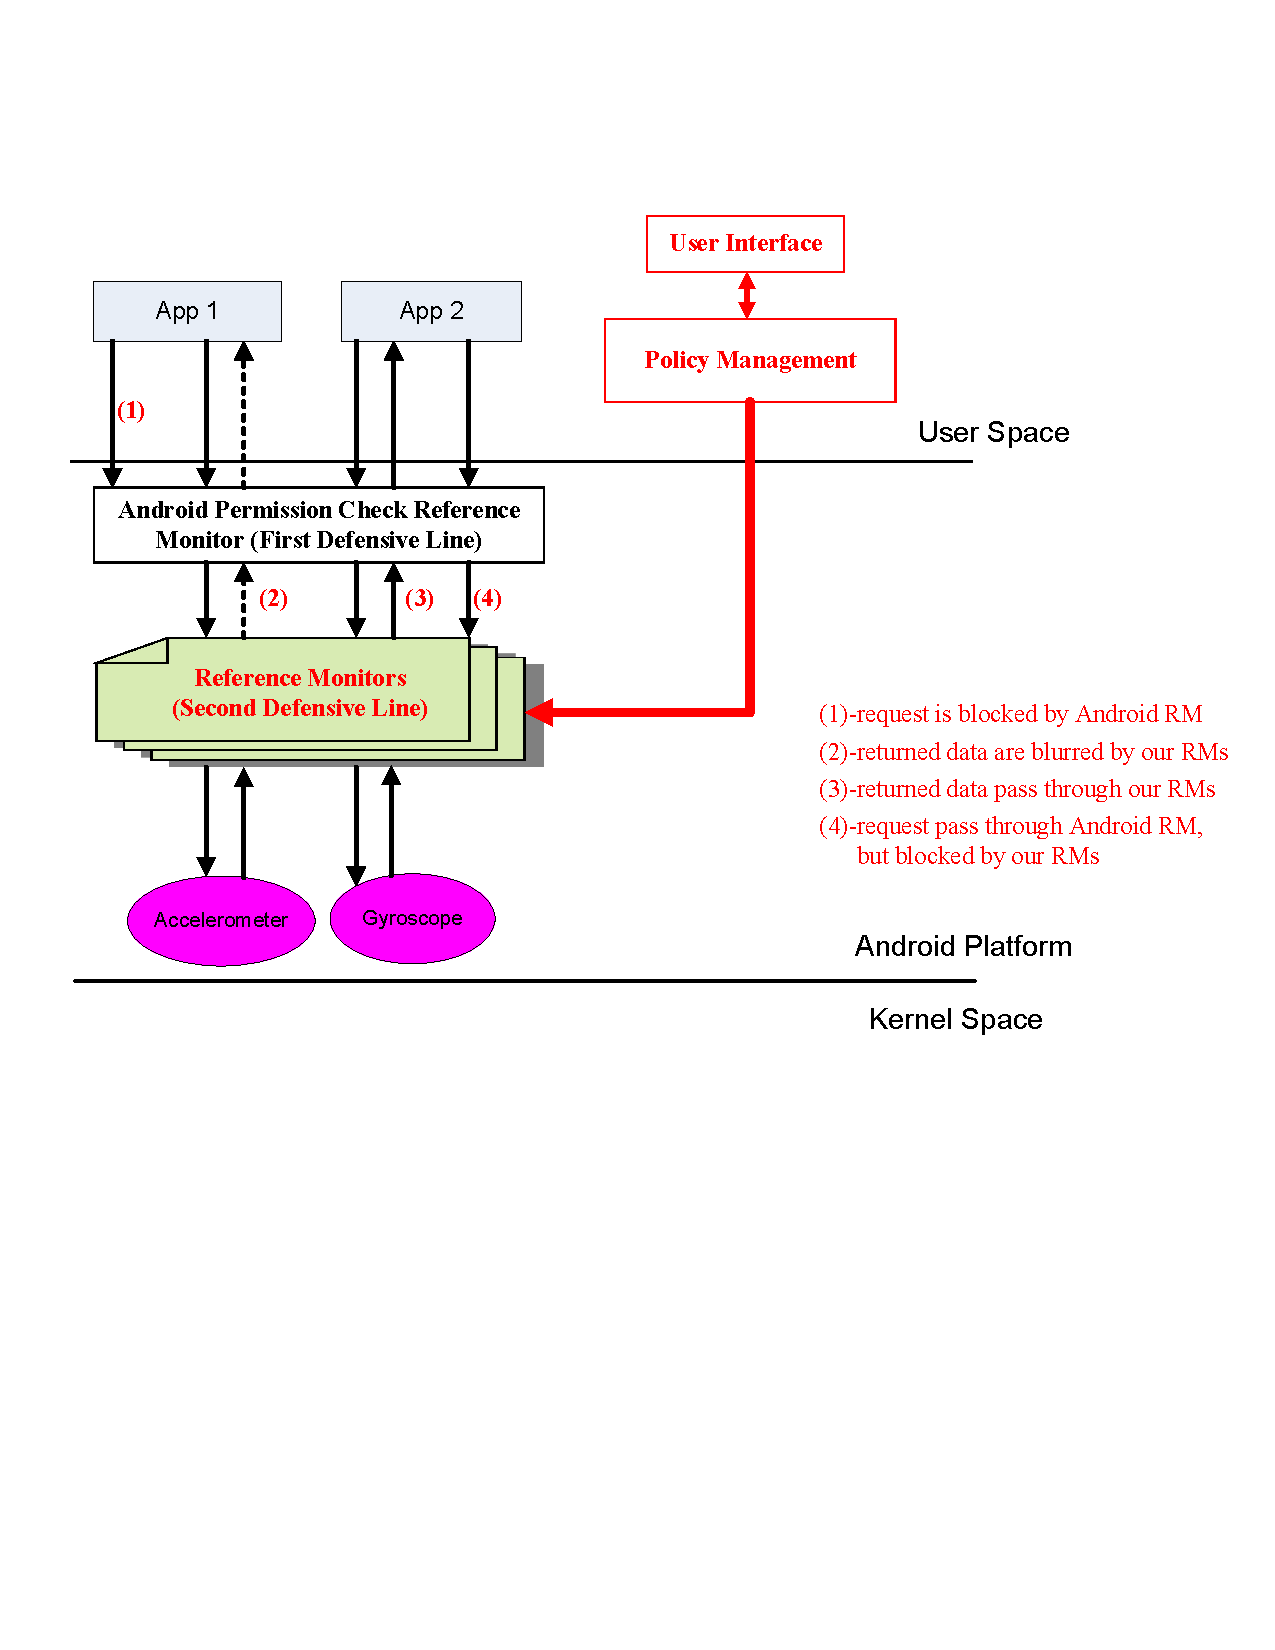
\includegraphics[width=3.7in]{refMonDesign.pdf}\\
  \caption{System architecture.}
  \label{Fig:design}
\end{figure}

The BlurSense project deals with this problem of fine-grained conrol of sensor data
by requiring that all untrusted apps be installed
through an app that filters sensor data through a reference monitor~\cite{cappos2014blursense}.  
(See Figure~\ref{Fig:design})
The level of trust is left up to the user.  The reference
monitor can exercise fine-grained control to degrade the accuracy of the sensor data, render it 
completely meaningless, or pass it through unchanged.  
In the case of geolocation, GPS measurements can be set to the center of the nearest
large city or random noise can be added.  
The second approach is to apply a trust metric, so that untrusted apps are denied access to certain
sensor data completely,
The reference monitor approach poses less risk than others; the worst that can happen is
that the app will have the same access to the sensor data that
is permitted by the manifest file. In the ideal case, Blursense
would limit the access to sensor data based on a trust metric for the app.

\weiss{this is redundant, but maybe we should say something}
Currently, implemented sensor modules and
the available contextual information are classified into three
categories: device specific (percentage of battery power level,
CPU and memory utility), location related (latitude, longitude,
altitude, accuracy, and speed if available), and network related
(mobile network type and operator, nearby WiFi access point
and Bluetooth devices). While sensor modules are the system
hooks with read access to valuable sensor resources, they
cannot manipulate sensor data. Additionally, the sensor API
also provides a base registry service with a common interface
for use by a sensor implementation. For both local and remote
processes to access sensor data, an json/sl4a library. \weiss{what do we want to say here?}
is incorporated to provide data in an unified format. In case
newer sensors appear on future mobile devices, developers can
add newly implemented sensors into this framework rather
easily. 
%The registry service listens for connection on a set of predefined ports via XML-RPC. 
Thus, both local and remote
process can connect to these ports and register for sensor
updates.
Our preliminary work in this area has resulted in working 
code~\cite{seattle-sensor-git}, tutorials~\cite{seattle-sensor-project}, and a 
blog for problem discussion~\cite{sensor}. Several different groups have
already used our early-stage proof-of-concept to solve problems across a variety
of domains, demonstrating the potential of sharing sensor data. 

\subsection{GPS Data}
\eat{
1) Overview of the Solution: Today's smartphone OS typ-
ically exposes resources based on a static policy. Such per-
missions are often much more than necessary. Several related
work has been proposed to refine or reduce permissions on
mobile platforms [18], [29], [17], [30] via modifying the
device platform. BlurSense allows untrusted parties to add
privacy filters from user space. Multiple security vendors
can efficiently and effectively collaborate to strengthen user
privacy.} %end comment

BlurSense provides a way to control the precision and accuracy of the GPS
sensor.  We show how blurring the GPS location affects the difference between
speed measured by a car speedometer and communicated via the OBD port to
a smartphone, similar to our experiment in section~\ref{sec:geolocation}.

\begin{figure}
\centering
%\includegraphics[width=3.5in]{}
\caption{Speed difference vs time with blurring of the GPS data.}
\label{fig:blur-GPS}
\end{figure}


\eat{
 BlurSense
provides a programmable privacy protection framework. Users
not only gain full transparency of what information is captured
on their devices, but also have full control over how much
information they would share with the rest of the world -
a secure personal data ecosystem. After installing BlurSense,
a user can install software from a third party (like a security vendor) that performs custom sensor filtering actions in
response to application requests. For example, an application
could be prevented from using motion sensors when running
in the background, or precise GPS data could be abstracted
to a neighborhood or zip code. 
BlurSense
provides effective controls for smartphones, much like Flash and JavaScript
filtering tools protect laptops and desktops (e.g., NoScript~\cite{noscript},
AdBlock~\cite{adblock}, FlashBlock~\cite{Flashblock}). 

2) What BlurSense Provides: Seattle provides a sensor
interposition mechanism and a sandboxing mechanism that
make it easy to implement privacy filters. A user can let a third
party have access to their sensor data from within a security
and performance isolated container [20]. By leveraging this
security, the user provides minimal trust in the third party,
but allows them an easy way to code their filters. This
functionality also automatically handles multiple privacy filters
from different parties through the sandbox policy composition
functionality~\cite{Cappos_CCS_10}.
Researchers who use BlurSense will build a mechanism
to trap the requests from generic  applications and pass them
into BlurSense (a proof-of-concept for Android has already
been built). They will build and manage an ``App Store'' for
BlurSense to allow users to locate privacy filters they wish
to apply. These may range from sharing sensor data with
researchers by reducing the precision of sensor values, salting
and hashing sensor values for anonymizing collected data,
or completely denying access to individual (or all) sensors.
For a particular sensor, a filter might perform an action such
as blurring the resolution of photos and video taken by the
camera, removing access point information from WiFi scans,
or omitting the motion sensor data completely. Security and
privacy groups can easily build and disseminate their own
privacy filters they recommend to users by adding them to
BlurSense app store. Therefore, BlurSense is able to handle
the three categories of threats in Section


\eat{To protect smartphone users'
privacy, Blursense provides a dynamic, fine-
grained, flexible access control mechanism, which incorporates
privacy filters in user space [19], [20]. } % end comment

We want to let users
choose defenses freely in a marketplace so that different
vendors can build them.
Specifically, it implements a framework of reference
monitors, to enforce mandatory access control to sensor data
in real time. A reference monitor is a method or function that
implements an access control policy for a set of resources and
is usually specified in terms of what capabilities are allowed.
The access control that we are concerned with in this paper is
for sensor data with respect to applications in user space. If
such an application needs to access any of the sensor data, the
second line of defensive (reference monitors) will come into
play, mediating every access to sensor data. 
%As a result, a user should be able to combine solutions from different vendors.
If a vendor's product is vulnerable to attack or the vendor is malicious,
the user can still be protected.
According to the semantics of the access requests and the
current context, when a remote procedure call is made to the
Android OS to request sensor data, it will be handled by a
reference monitor. Based on a sensitivity of the application,
the data returned may be filtered, dropped or passed through.
Note that the reference monitor cannot pass on data that is
blocked by the manifest file because it is layered on top of
whatever privacy and security mechanisms that are in place at
the OS level. If the request is for highly sensitive sensor data,
then the request might be simply rejected. Otherwise, if the
request is for medium-level sensitive sensor data, the request
might get through, but the returned data has reduced resolution.
If the request is for low-sensitive sensor data, then the return
results need to be processed, e.g., by filtering or obfuscation.
BlurSense can be used with Sensibility Testbed~\cite{cappos-sensibility}, 
which provides
a rich and extensible collection of sensor data from Android
devices 
}
